\subsection{تولید شرح بر تصاویر با استفاده از روش‌های مبتنی بر نقطه توجه}
ایده‌ اصلی روش‌های مبتنی بر نقطه توجه از پژوهش‌های موجود در زمینه ترجمه ماشینی گرفته شده است. این دسته از پژوهش‌ها مدلی ارائه می‌دهند که با استفاده از آن بتوان هر کلمه از جملات تولیدی را با تمرکز بر یک یا بخشی از کلمات موجود در جمله مبدا‌، تولید کرد. به طور مشابه، در حوزه تولید خودکار شرح بر تصاویر، از این دسته از پژوهش‌ها به منظور حصول مدلی استفاده می‌شود که قادر باشد هر یک از کلمات موجود در جمله را با استفاده از بخشی از تصویر ورودی، تولید نماید.
\\
در این فصل، ابتدا ایده اصلی ترجمه مبتنی بر نقطه توجه را در حوزه ترجمه ماشینی ارائه خواهیم کرد و سپس کاربردهای این ایده را در حوزه تولید خودکار شرح بر تصاویر مورد بررسی قرار می‌دهیم. 

\subsection{روش‌های مبتنی بر نقطه توجه در حوزه ترجمه ماشینی}

همان‌طور که گفته شد، تمام روش‌های قبلی را می‌توان به دو مرحله زیر تقسیم کرد.
\begin{enumerate}
\item نگاشت نمونه‌ها از فضای تصاویر به فضای ویژگي‌ها
\item نگاشت نمونه‌ها از فضای ویژگی‌ها به فضای جملات
\end{enumerate}

در حوزه ترجمه ماشینی، به تابع نگاشت مرحله اول، انکودر\enfootnote{Encoder} و به تابع نگاشت مرحله دوم، دیکودر\enfootnote{Decoder} گفته می‌شود. در این بخش، ما از این عبارات برای ارجاع به مراحل اول و دوم الگوریتم استفاده می‌نماییم.
\\
چارچوب کاری انکودر-دیکودر، در تعداد زیادی از پژوهش‌های حوزه ترجمه ماشینی به عنوان چارچوب کاری اصلی مورد استفاده قرار گرفته است. تمام روش‌های قبلی که در فصول قبل ذکر شد نیز از همین چارچوب کاری به عنوان چارچوب اصلی بهره برده‌اند. به عنوان مثال در روش‌های مبتنی بر یادگیری عمیق برای تولید خودکار شرح بر تصاویر از شبکه‌های عصبی کانولوشنی به طور معمول به عنوان انکودر و از شبکه‌های عصبی بازگشتی به عنوان دیکودر استفاده می‌شود.
\\
شکل \ref{fig:5-1} نشان‌دهنده ساختار کلی چارچوب کاری انکودر-دیکودر است.

\begin{figure}[h]
\centering
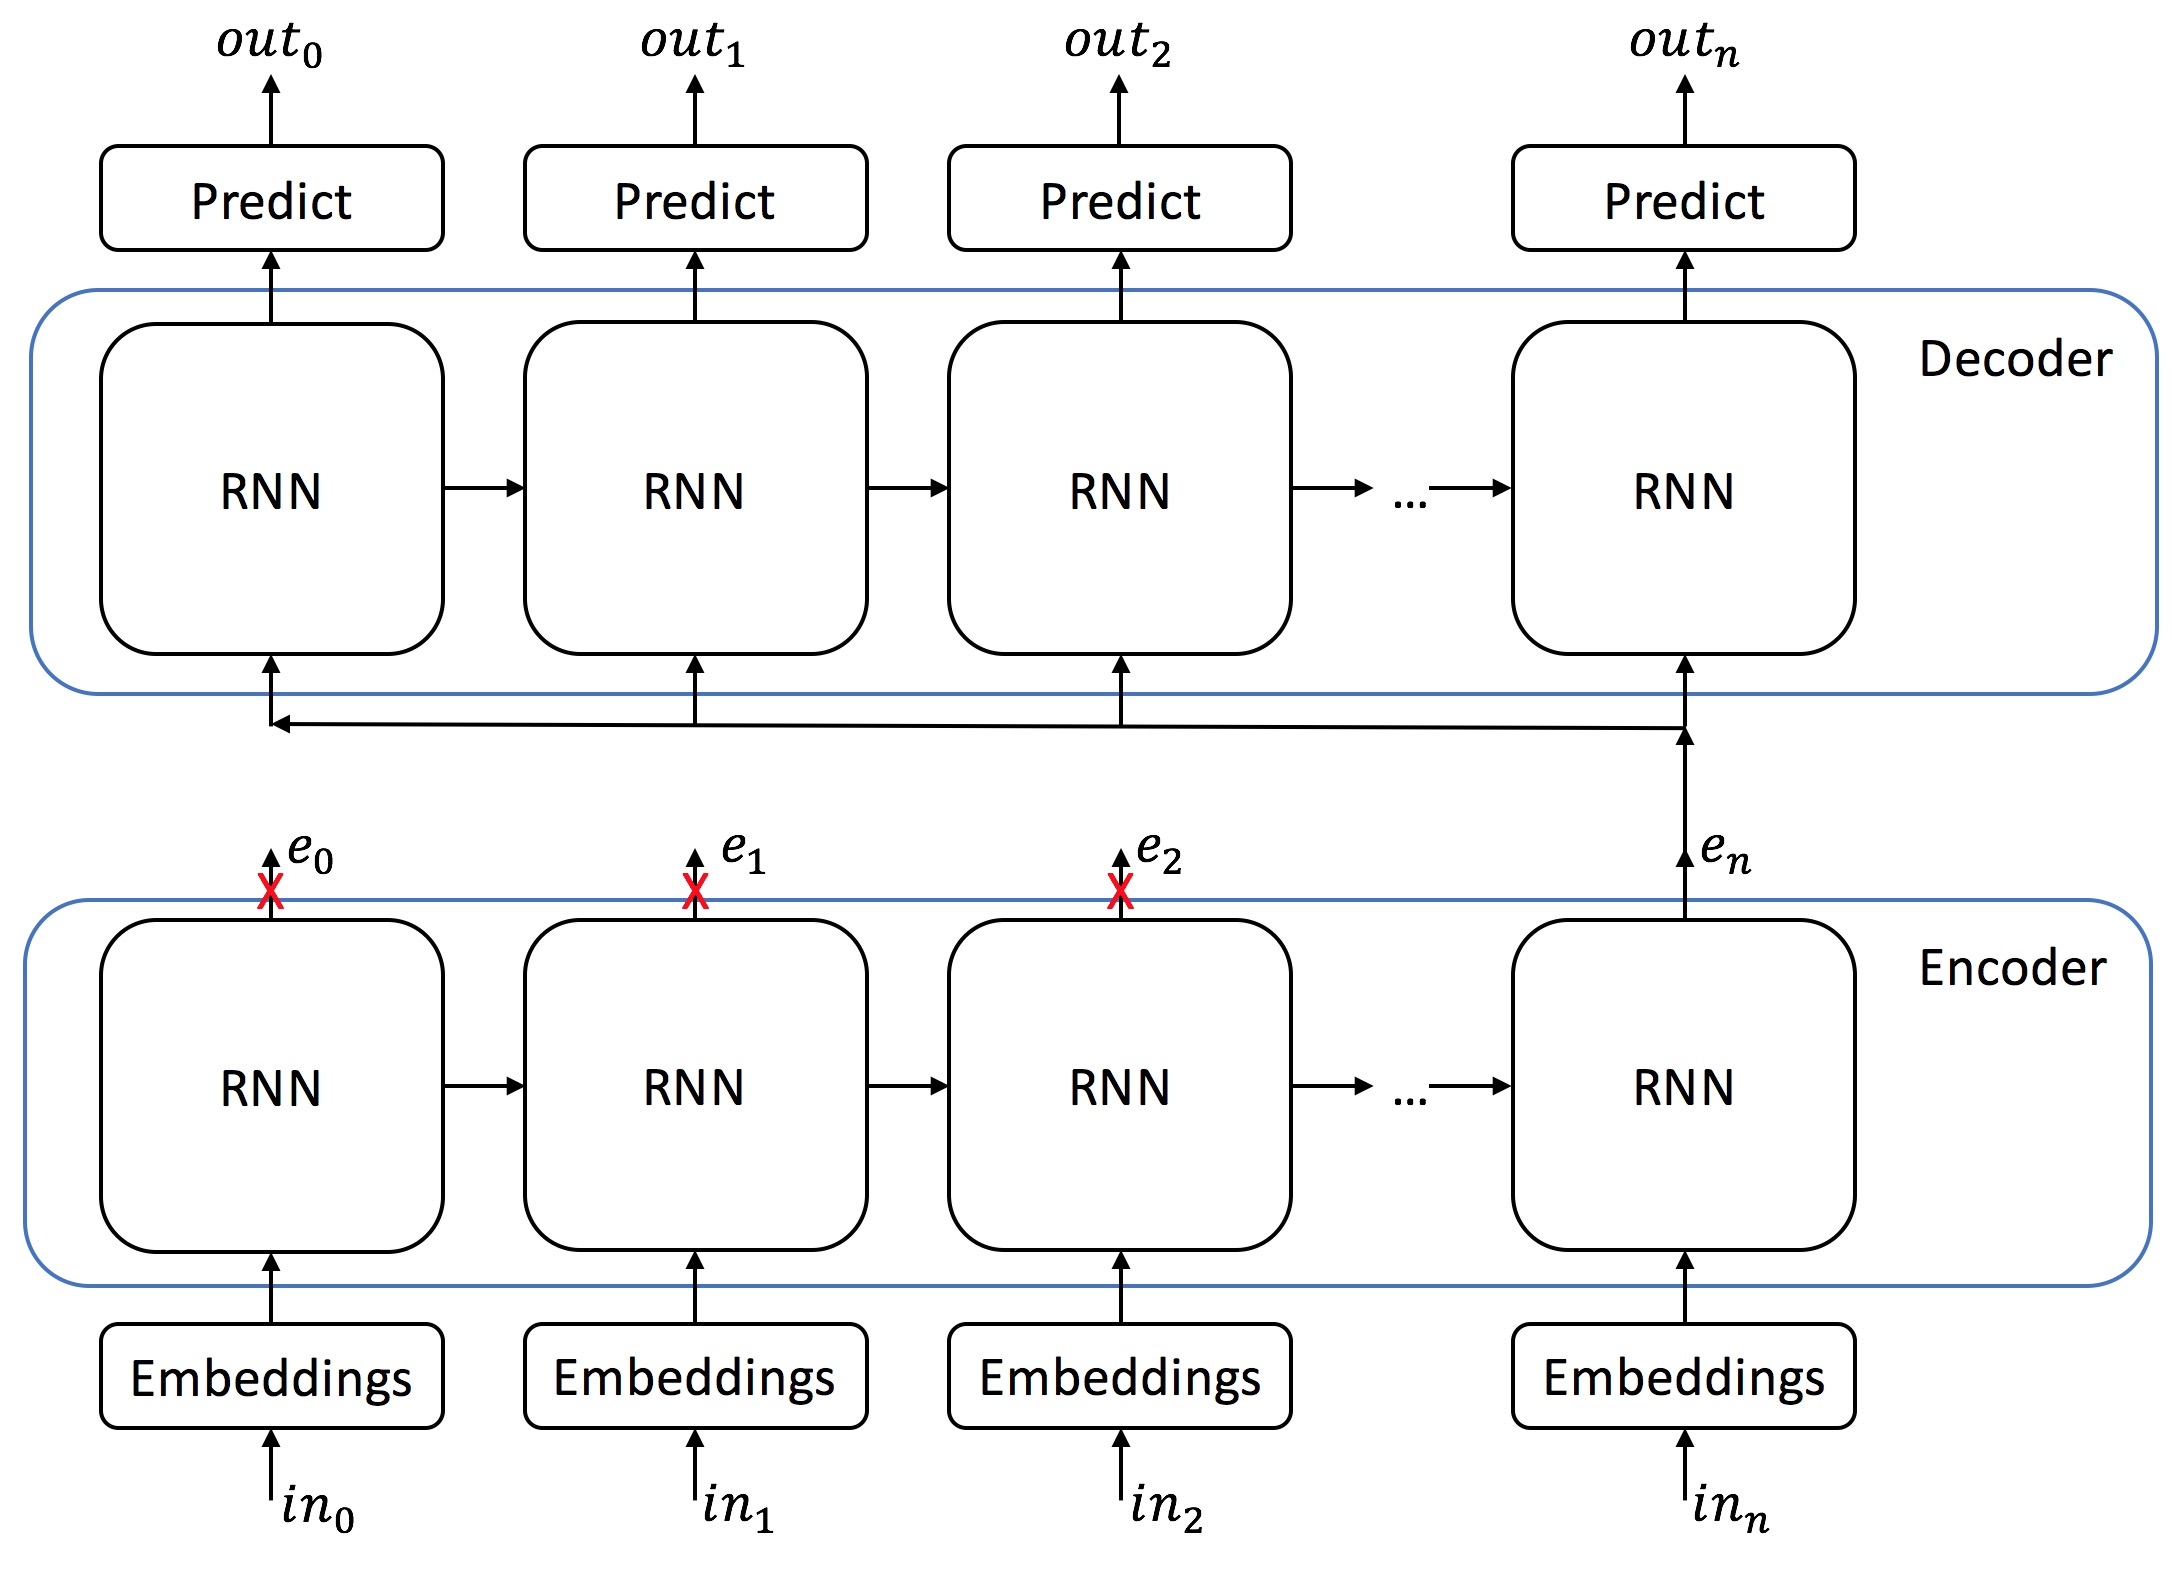
\includegraphics[scale=0.4]{Imgs/encoder-decoder.jpg}
\caption{ساختار کلی چارچوب کاری انکودر-دیکودر}
\label{ref:fig:5-1}
\end{figure}


در ادامه به بررسی بخش‌های مختلف این چارچوب کاری می‌پردازیم و سپس ایده اصلی روش‌های مبتنی بر نقطه توجه را که توسط آقای بنجیو در پژوهش \cite{bahdanau2014neural} در سال 2014 ارائه شده است، مورد بررسی قرار خواهیم 
داد.


\subsubsection{انکودر}
 انکودر در این چارچوب کاری، با گرفتن یک جمله به عنوان ورودی، بردار ویژگی متناظر جمله مبدا را تولید می‌کند. جمله ورودی با دنباله‌ای از کلمات مدل می‌شود. همین‌طور هر کلمه را با یک بردار $n$ بعدی، که $n$ تعداد کلمات موجود در دیکشنری است، مدل می‌شود. به این ترتیب، هر جمله ورودی، یک بردار با طول متغیر است که هر مولفه آن خودش برداری به ابعاد  $n$ است. از طرفی بردار خروجی، که همان بردار ویژگی‌ها است، یک بردار با طول ثابت و قراردادی خواهد بود.
 \\
 عموما در کاربردهای ترجمه ماشینی در هر دو بخش انکودر و دیکودر از شبکه‌های عصبی بازگشتی استفاده می‌شود. در شبکه‌های عصبی بازگشتی، خروجی هر مرحله تابعی از ورودی آن مرحله و حالت شبکه در مرحله جاری است. با فرض این‌که $h_t$ حالت شبکه در زمان $t$ را نمایش دهد می‌توان رابطه تولید خروجی توسط شبکه عصبی بازگشتی را مطابق با \eqref{eq:5-1} تعریف نمود.
\begin{align*}
h_t& = f(X_t , h_{t-1}) \\
C& = q(h_1, \cdots, h_L)
\numberthis 
\label{eq:5-1}
\end{align*}
به طور معمول از شبکه 
\lr{LSTM}
 به عنوان تابع $f$ استفاده می‌شود و همین‌طور به جای استفاده از تابع $q$ حالت نهایی شبکه به عنوان بردار ویژگی مورد استفاده قرار می‌گیرد
\cite{bahdanau2014neural}.

\subsubsection{دیکودر}

 دیکودر به منظور نگاشت فضای ویژگی‌ها به فضای جملات مورد استفاده قرار می‌گیرد. خروجی انکودر، ورودی دیکودر است. با این فرض، ورودی دیکودر یک بردار ویژگی با طول ثابت است و خروجی آن که یک جمله به زبان مقصد است، همانند جمله مبدا، یک بردار با طول متغیر شامل بردارهای بازنمایی کلمات است. دیکودر در اصل در هر مرحله، به دنبال یافتن کلمه‌ای است که با داشتن کلمات تولید شده قبلی و بردار ویژگی موجود، محتمل‌ترین کلمه نسبت به بقیه کلمات موجود در دیکشنری باشد. تابع احتمال مربوطه را می‌توان به فرم \eqref{eq:5-2} تعریف نمود.
 
 \begin{equation}
 p(y_t | C, y_1, y_2, \cdots, y_{t-1}) = g(y_t, s_t, C)
 \label{eq:5-2}
 \end{equation}

در رابطه \eqref{eq:5-2}، $C$ نشان‌دهنده بردار ویژگی‌، $y_i$ نشان‌دهنده لغت $i$ام تولید شده از زبان مقصد و بردار $s_t$ نشان‌دهنده حالت شبکه بازگشتی مورد استفاده به عنوان دیکودر است.


 شکل \ref{fig:decoder} ساختار کلی دیکودر را نمایش می‌دهد.

\begin{figure}[h]
\centering
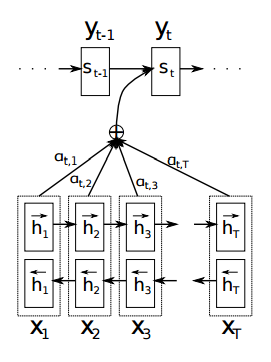
\includegraphics[scale=0.7]{Imgs/5-decoder.png}
\caption{ساختار دیکودر مورد استفاده در چارچوب کاری \cite{bahdanau2014neural}}
\label{fig:decoder}
\end{figure}

\subsubsection{ایده اصلی استفاده از نقطه توجه}

همان‌طور که بیان شد، در چارچوب کاری انکودر-دیکودر، ابتدا جمله ورودی که شامل تعداد نامعلوم کلمه است به یک بردار با طول متغیر مدل می‌شود. بردار تولید شده توسط یک انکودر به یک بردار با طول ثابت، که همان بردار ویژگی‌ها است، نگاشت شده و در نهایت بردار ویژگی تولید شده توسط یک انکودر به یک بردار با طول متغیر که نماینده جمله زبان مقصد است، نگاشت می‌شود.
\\
فرآیند مذکور یک محدودیت جدی دارد و آن این است که انکودر باید بتواند تمام اطلاعات مورد نیاز برای تولید جمله را در یک بردار با طول ثابت بگنجاند و دیکودر باید بتواند تمام اطلاعات مورد نیاز خود را از همین بردار با موجود با طول ثابت، استخراج کند. این محدودیت باعث می‌شود قدرت کد کردن اطلاعات در بردار ویژگی کاهش یابد. برای حل این مشکل از ایده نقاط توجه استفاده می‌نماییم.
\\
در این دسته از روش‌ها به جای این‌که انکودر فقط یک بردار ویژگی تولید کند، بردارهای ویژگی مختلفی ایجاد می‌کند که هر بردار با تمرکز بر روی یک یا بخشی از جمله مبدا تولید شده است. به این ترتیب، هر بردار تولید شده شامل اطلاعات معنایی یک یا بخشی از جمله مبدا می‌باشد. به این طریق، دیکودر می‌تواند با انتخاب بین بردارهای معنایی تولید شده در هر مرحله، کلمه تولیدی را با تمرکز بر روی معنای یک کلمه و کلمات مجاور آن در جمله مبدا، تولید کند.
\\
در ادامه به بررسی تغییراتی که باید در انکودر و دیکودر اتفاق بیفتد تا بتوان به جای یک بردار ویژگی مجموعه‌ای از بردارهای ویژگی با تمرکز محلی ایجاد نمود و از آن‌ها برای تولید جمله استفاده نمود را مورد بررسی قرار می‌دهیم. برای سهولت فهم تغییرات، ابتدا تغییرات دیکودر را مطرح نموده و سپس به بررسی تغییرات انکودر خواهیم پرداخت.
\subsubsection{دیکودر در روش مبتنی بر نقطه توجه}
فرض می‌کنیم به جای تنها یک بردار ویژگی، $L$ بردار ویژگی از ورودی استخراج شده باشد. آن‌ها را در یک ماتریس به شکل $C = [c_1, \cdots, c_L]^T$ بازنمایی می‌نماییم. فرض می‌کنیم بردار ویژگی $c_i$ به دنباله حاشیه‌نویسی‌های\enfootnote{Annotation} $h = [h_1, \cdots, h_L]^T$ وابسته است. حاشیه‌نویسی $h_i$ خود یک متغیر تصادفی به شکل برداری است که دارای دو ویژگی بسیار مهم می‌باشد.
\begin{enumerate}
\item .حاوی اطلاعات استخراج شده از تمام جمله است
\item تمرکز استخراج اطلاعات بر روی کلمه $i$ام و کلمات اطراف آن بوده است.
\end{enumerate}
با تعریف این دو ویژگی، حاشیه‌نویسی‌ها را می‌توان همان بردار ویژگی جمله تصور کرد با این شرط که علاوه بر این که معنای کل جمله را کد کرده‌اند، تمرکز بیشتری بر معنای کلمه $i$ام و کلمات مجاور آن دارند. به عبارت بهتر هر حاشیه‌نویسی علاوه بر این‌که معنای کلی جمله را کد می‌کند، حاوی معنای محلی مربوط به کلمات هم هست.
\\
با تعریف حاشیه‌نویسی به شکل فوق و با تکیه بر فرض‌های انجام شده، می‌توانیم مدل احتمالاتی ارائه شده را به شکل  \eqref{eq:5-3} تغییر دهیم. 
\begin{equation}
p(y_i| y_1, \cdots, y_{i-1}, X) = g(y_{i-1}, S_i, c_i)
\label{eq:5-3} 
\end{equation}
که در آن:
\begin{align*}
c_i = \Sigma_{j=1}^L \alpha_{ij}h_j
\numberthis
\label{eq:5-4}
\\
\alpha_{ij} = \frac{exp(e_{ij})}{\Sigma_{k=1}^Lexp(e_{ik})}
\numberthis
\label{eq:5-5}
\\
e_{ij} = f(s_{i-1}, h_j)
\numberthis
\label{eq:5-6}
\end{align*}

متغیر تصادفی $e_{ij}$ که در رابطه \eqref{eq:5-6} تعریف شده است نمایان‌گر میزان شباهت کلمه $i$ام در جمله خروجی به کلمه $j$ام در جمله ورودی است. وظیفه‌ این متغیر، هم‌ترازسازی\enfootnote{Alignment} ورودی و خروجی است. $\alpha_{ij}$ یک نرمال‌سازی روی امتیازهای محاسبه شده انجام می‌دهد. از این متغیر نرمال شده به عنوان وزن حاشیه‌نویسی‌ها استفاده می‌شود. مطابق با رابطه \eqref{eq:5-4} بردار ویژگی مورد استفاده برای تولید کلمه در جمله مقصد، از طریق یک میانگین‌گیری بر اساس وزن معنایی کلمات تولید می‌شود.
\\
در رابطه \eqref{eq:5-6} $s_{i-1}$ بردار حالت شبکه دیکودر در زمان $i-1$ و $f$ یک تابع امتیاز است. تابع امتیاز مورد استفاده در این رابطه را می‌توان با یک شبکه عصبی پیش‌رو\enfootnote{Feed Forward Neural Network} مدل‌سازی کرد. در صورت استفاده از شبکه عصبی پیش‌رو برای مدل‌سازی تابع شباهت، در صورتی که از هم‌ترازسازی نرم\enfootnote{Soft Alignment} استفاده شود، تابع هدف مشتق‌پذیر شده و می‌توانیم از الگوریتم پس‌انتشار خطا برای آموزش استفاده نماییم.


\subsubsection{انکودر در روش مبتنی بر نقطه توجه}
برای طراحی انکودر در این بخش، باید مکانیزمی ارائه شود که قادر باشد حاشیه‌نویسی‌های $h_1$ تا $h_L$ را طوری تولید کند که دو شرط مطرح شده در بخش قبلی را ارضا نمایند. به عبارت دیگر باید بردارهای ویژگی‌ای استخراج نماییم که علاوه بر این‌که حاوی معنای کل جمله باشند، هر یک از آن‌ها بر روی معنای یک کلمه و کلمات اطراف آن تمرکز بیشتری نسبت به سایر بردارها داشته باشند تا بتوانیم علاوه بر مدل‌سازی معنای کلی جمله، از معنای محلی کلمات هم استفاده نماییم.
\\
به این منظور از یک شبکه عصبی بازگشتی دوطرفه در مدل‌سازی انکودر استفاده می‌نماییم. شکل \ref{fig:biencoder} ساختار کلی یک شبکه عصبی بازگشتی دوطرفه را نمایش می‌دهد. 

\begin{figure}[h]
\centering
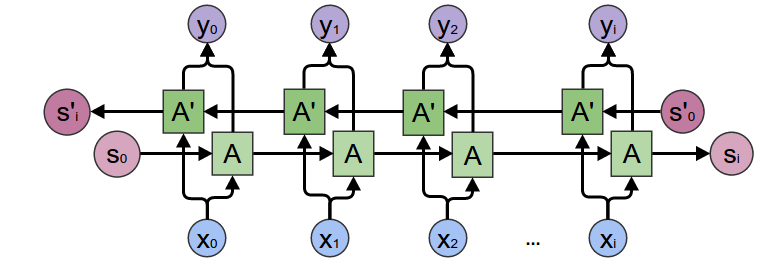
\includegraphics[scale=0.6]{Imgs/biencoder.png}
\caption{ساختار کلی یک شبکه عصبی بازگشتی دوطرفه}
\label{fig:biencoder}
\end{figure}

همان‌طور که در شکل \ref{fig:biencoder} مشخص است، یک شبکه عصبی بازگشتی دوطرفه شامل دو شبکه پیش‌رو در خلاف جهت یک‌دیگر است. حالت‌های مخفی شبکه پیش‌رو رو به راست را با $h_i^\rightarrow$ و حالت‌های مخفی شبکه پیش‌رو رو به چپ را با $h_i^\leftarrow$ نمایش می‌دهیم. همان‌طور که در شکل پیداست، خروجی‌های شبکه در این ساختار هم به حالت‌های سمت راست و کلمات سمت راست در جمله و هم به حالات و کلمات سمت چپ وابسته هستند. پس همین خروجی‌ها را می‌توان به عنوان حاشیه‌نویسی‌هایی که هر دو ویژگی را دارند مورد استفاده قرار داد.
	











